\documentclass[12pt,a4paper]{article}

% 导入必要的宏包
\usepackage[UTF8]{ctex}
\usepackage{geometry}
\usepackage{amsmath}
\usepackage{amsfonts}
\usepackage{amssymb}
\usepackage{graphicx}
\usepackage{enumitem}
\usepackage{xcolor}
\usepackage{tikz}
\usepackage{float}
\usepackage{hyperref}
\usepackage{multicol}
\usepackage{longtable}
\usepackage{array}
\usepackage{tabularx}
\usepackage{listings}

% 代码高亮设置
\lstset{
    basicstyle=\ttfamily,
    keywordstyle=\color{blue},
    commentstyle=\color{green},
    stringstyle=\color{red}
}

% 页面设置
\geometry{left=2.5cm,right=2.5cm,top=2.5cm,bottom=2.5cm}

% 标题页设置
\title{\textbf{2023年数据结构题库} \\ \large }
\author{}
\date{}

% 定义题型环境
\newenvironment{choicequestion}[1][]{%
    \vspace{0.5cm}
    \noindent\textbf{[#1]}
    \vspace{0.2cm}
}{}

\newenvironment{answersection}{%
    \vspace{0.2cm}
    \noindent\textbf{[参考答案]}\\
    \vspace{0.1cm}
}{}

\newenvironment{analysissection}{%
    \vspace{0.2cm}
    \noindent\textbf{[答案解析]}\\
    \vspace{0.1cm}
}{}

% 定义题号计数器
\newcounter{questioncounter}

% 问题格式化命令
\newcommand{\question}[2]{%
    \stepcounter{questioncounter}%
    \noindent\textbf{\thequestioncounter} #1%
}

% 选择题选项格式
\newcommand{\choices}[4]{%
    \begin{multicols}{2}
    \noindent \textbf{A.} #1 \par
    \noindent \textbf{B.} #2 \par
    \noindent \textbf{C.} #3 \par
    \noindent \textbf{D.} #4 \par
    \end{multicols}%
}

% 表格格式
\newcolumntype{Y}{>{\centering\arraybackslash}X}

% 开始文档
\begin{document}

\maketitle

\section{单项选择题}

\begin{choicequestion}[单选题]
\question{下列对顺序存储的有序表（长度为 $n$ ）实现给定操作的算法中，平均时间复杂度为 $O(1)$ 的是（）。}{D}
\choices{查找包含指定值元素的算法}{插入包含指定值元素的算法}{删除第 $i(1 \leqslant i \leqslant n)$ 个元素的算法}{获取第 $i$ （ $1\leqslant i\leqslant n$ ）个元素的算法}}

\begin{answersection}
D. 获取第 $i$ （ $1\leqslant i\leqslant n$ ）个元素的算法
\end{answersection}

\begin{analysissection}
顺序存储的有序表中，获取第i个元素可以直接通过数组下标访问，时间复杂度为O(1)。其他操作都需要涉及搜索或移动元素，时间复杂度更高。
\end{analysissection}
\end{choicequestion}

\begin{choicequestion}[单选题]
\question{现有非空双向链表 L, 其结点结构为: prev data next, prev 是指向直接前驱结点的指针, next 是指向后继结点的指针。若要在 L 中指针 p 所指向的节点 (非尾结点) 之后插入指针 s 指向的新结点, 则在执行了语句序列 "s -> next = p -> next; p -> next = s" 后, 下列语句序列中还需要执行的是 ( )。}{C}
\choices{s -> next -> prev = p; s -> prev = p;}{p->next->prev = s; s->prev = p;}{s \rightarrow \text{prev} = s \rightarrow \text{next} \rightarrow \text{prev}; s \rightarrow \text{next} \rightarrow \text{prev} = s;}{p \rightarrow next -> prev = s -> prev; s \rightarrow next -> prev = p;}}

\begin{answersection}
C. s \rightarrow \text{prev} = s \rightarrow \text{next} \rightarrow \text{prev}; s \rightarrow \text{next} \rightarrow \text{prev} = s;
\end{answersection}

\begin{analysissection}
在双向链表中插入节点s到p之后，需要设置s的prev指针指向p，并设置s->next的prev指针指向s。已完成的是s->next=p->next和p->next=s，还需要设置s->prev=p和s->next->prev=s。
\end{analysissection}
\end{choicequestion}

\begin{choicequestion}[单选题]
\question{若采用三元组表存储结构存储稀疏矩阵 M，则除三元组表外，下列数据中还需要保存的是（）。\newline
I. M的行数\newline
II. M中包含非零元素的行数\newline
III.M的列数\newline
IV.M中包含非零元素的列数}{A}
\choices{仅 I、III}{仅 I、IV}{仅 II、IV}{I、II、III、IV}}

\begin{answersection}
A. 仅 I、III
\end{answersection}

\begin{analysissection}
三元组表存储稀疏矩阵时，需要知道矩阵的行数和列数以确定矩阵的整体结构，而不仅仅是非零元素的行列数。
\end{analysissection}
\end{choicequestion}

\begin{choicequestion}[单选题]
\question{在由 6 个字符组成的字符集 S 中, 各字符出现的频次分别为 3, 4, 5, 6, 8, 10, 为 S 构造的哈夫曼编码的加权平均长度为 ( )。}{B}
\choices{2.4}{2.5}{2.67}{2.75}}

\begin{answersection}
B. 2.5
\end{answersection}

\begin{analysissection}
构建哈夫曼树，计算带权路径长度。总频次=3+4+5+6+8+10=36。通过构造哈夫曼树得到各字符的编码长度，然后计算加权平均长度。
\end{analysissection}
\end{choicequestion}

\begin{choicequestion}[单选题]
\question{已知一棵二叉树的树形如右图所示，若其后序遍历序列为 f, d, b, e, c, a，则其先（前）序遍历序列是（）。}{A}

\begin{figure}[H]
\centering
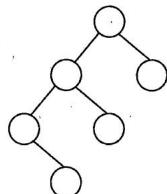
\includegraphics[width=0.3\textwidth]{images/bbead846e08c25bd9b1ef0f9c3134f75fa306d74b5d2054eb876fa93c3796a0a.jpg}
\end{figure}

\choices{a, e, d, f, b, c}{a, c, e, b, d, f}{c, a, b, e, f, d}{d, f, e, b, a, c}}

\begin{answersection}
A. a, e, d, f, b, c
\end{answersection}

\begin{analysissection}
根据后序遍历序列f, d, b, e, c, a和树的形状，可以确定树的结构，从而得到先序遍历序列。
\end{analysissection}
\end{choicequestion}

\begin{choicequestion}[单选题]
\question{已知无向连通图 G 中各边的权值均为 1。下列算法中，一定能够求出图 G 中从某顶点到其余各个顶点最短路径的是（）。\newline
I.普里姆（Prim）算法\newline
II. 克鲁斯卡尔（Kruskal）算法\newline
III. 广度优先搜索算法}{B}
\choices{仅 I}{仅 III}{仅 I、II}{I、II、III}}

\begin{answersection}
B. 仅 III
\end{answersection}

\begin{analysissection}
只有广度优先搜索算法能求出从某顶点到其余各顶点的最短路径。Prim和Kruskal是用于求最小生成树的算法。
\end{analysissection}
\end{choicequestion}

\begin{choicequestion}[单选题]
\question{下列非空 $B$ 树的叙述中，正确的是（）。\newline
I. 插入操作可能增加树的高度\newline
II. 删除操作一定会导致叶结点的变化\newline
III.查找某关键字总是要查找到叶结点\newline
IV.插入的新关键字最终位于叶结点中}{A}
\choices{仅 I}{仅 I、II}{仅 III、IV}{仅 I、II、IV}}

\begin{answersection}
A. 仅 I
\end{answersection}

\begin{analysissection}
I. 正确，当节点分裂传播到根节点时，B树高度会增加。
II. 错误，删除操作不一定导致叶节点变化。
III. 错误，查找可能在内部节点找到。
IV. 错误，插入的关键字可能在内部节点。
\end{analysissection}
\end{choicequestion}

\begin{choicequestion}[单选题]
\question{对含有 600 个元素的有序顺序表进行折半查找, 关键字间的比较次数最多是 ( )。}{B}
\choices{9}{10}{30}{300}}

\begin{answersection}
B. 10
\end{answersection}

\begin{analysissection}
折半查找的最大比较次数为⌊log₂n⌋+1，对于600个元素，⌊log₂600⌋+1=⌊9.23⌋+1=9+1=10。
\end{analysissection}
\end{choicequestion}

\begin{choicequestion}[单选题]
\question{现有长度为 5, 初始为空的散列表 HT, 散列表函数 $H(k) = (k + 4)\% 5$ , 用线性探查再散列法解决冲突。若将关键字序列 2022, 12, 25 依次插入 HT 中, 然后删除关键字 25, 则 HT 中查找失败的平均查找长度为( )。}{D}
\choices{1}{1.6}{1.8}{2.2}}

\begin{answersection}
D. 2.2
\end{answersection}

\begin{analysissection}
计算过程：
H(2022)=(2022+4)%5=2026%5=1
H(12)=(12+4)%5=16%5=1(冲突，放到2)
H(25)=(25+4)%5=29%5=4
删除25后，表中位置1放2022，位置2放12。
查找失败时，需要探查到空位置。
\end{analysissection}
\end{choicequestion}

\begin{choicequestion}[单选题]
\question{下列排序算法中，不稳定的是（）。\newline
I. 希尔排序\newline
Ⅱ. 归并排序\newline
III. 快速排序\newline
IV.堆排序\newline
V. 基数排序}{C}
\choices{仅 I、II}{仅 II、V}{仅 I、III、IV}{仅 III、IV、V}}

\begin{answersection}
C. 仅 I、III、IV
\end{answersection}

\begin{analysissection}
归并排序和基数排序是稳定排序算法，希尔排序、快速排序和堆排序是不稳定排序算法。
\end{analysissection}
\end{choicequestion}

\begin{choicequestion}[单选题]
\question{使用快速排序算法对数据进行升序排序，若经过一次划分后得到的数据序列是68，11，70，23，80，77，48，81，93，88，则该次划分的枢轴是（）。}{C}
\choices{11}{70}{80}{81}}

\begin{answersection}
C. 80
\end{answersection}

\begin{analysissection}
在快速排序的一次划分后，枢轴元素应该在其最终的排序位置，左边的元素都小于等于它，右边的元素都大于等于它。序列68，11，70，23，80，77，48，81，93，88中，80左边的元素都小于等于80，右边的元素都大于等于80。
\end{analysissection}
\end{choicequestion}

\section{综合应用题}

\begin{choicequestion}[问答题]
\question{(13分)已知有向图G采用邻接矩阵存储，类型定义如下：\newline

\begin{lstlisting}[language=C]
typedef struct { // 图的类型定义
int numVertices, numEdges; // 图的顶点数和有向边数
char VerticesList[MAXV]; // 顶点表，MAXV为已定义常量
int Edge[MAXV][MAXV]; // 邻接矩阵
} MGraph;
\end{lstlisting}\newline

将图中出度大于入度的顶点称为K顶点。例如：在右图中，顶点a和顶点b都是K顶点。请设计算法：int printVertices(MGraph G)，对任意给定的非空有向图G，输出图G中所有的K顶点，并返回K顶点的个数。要求：\newline

\begin{figure}[H]
\centering
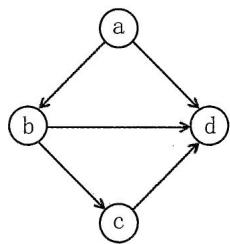
\includegraphics[width=0.3\textwidth]{images/72b8afcd4bb90ccbf66fba66340629da25258a3d10122ea61cb91608e788c8d0.jpg}
\end{figure}\newline

(1) 给出算法的基本设计思想。\newline
(2) 根据设计思想，采用 C 或 $\mathbf{C} + +$ 语言描述算法，关键之处给出注释。}{}

\begin{answersection}
(1) 算法的基本设计思想：
遍历图的每个顶点，计算每个顶点的入度和出度。入度是邻接矩阵中该顶点对应列中值为1的元素个数，出度是该顶点对应行中值为1的元素个数。然后比较每个顶点的出度和入度，如果出度大于入度，则该顶点为K顶点。

(2) 算法实现：
\end{answersection}

\begin{analysissection}
#include <stdio.h>

int printVertices(MGraph G) {
    int count = 0;  // K顶点计数
    
    // 遍历每个顶点
    for (int i = 0; i < G.numVertices; i++) {
        int inDegree = 0;    // 入度
        int outDegree = 0;   // 出度
        
        // 计算顶点i的出度（邻接矩阵第i行中值为1的元素个数）
        for (int j = 0; j < G.numVertices; j++) {
            if (G.Edge[i][j] == 1) {
                outDegree++;
            }
        }
        
        // 计算顶点i的入度（邻接矩阵第i列中值为1的元素个数）
        for (int k = 0; k < G.numVertices; k++) {
            if (G.Edge[k][i] == 1) {
                inDegree++;
            }
        }
        
        // 如果出度大于入度，则为K顶点
        if (outDegree > inDegree) {
            printf("K vertex: %c\n", G.VerticesList[i]);  // 输出K顶点
            count++;  // 计数器加1
        }
    }
    
    return count;  // 返回K顶点个数
}
\end{analysissection}
\end{choicequestion}

\begin{choicequestion}[问答题]
\question{(10分)对含有 $n(n > 0)$ 个记录的文件进行外部排序，采用置换-选择排序生成初始归并段时需要使用一个工作区，工作区中能保存 $m$ 个记录，请回答下列问题：\newline
(1) 若文件中有 19 个记录, 其关键字依次是 51, 94, 37, 92, 14, 63, 15, 99, 48, 56, 23, 60, 31, 17, 43, 8, 90, 166, 100。当 $m = 4$ 时, 可生成几个初始归并段? 每个归并段各是什么?  \newline
(2) 对任意 $m (n \gg m > 0)$ ，生成的第一个初始归并段的长度最大值和最小值分别是多少？}{}

\begin{answersection}
(1) 当m=4时，使用置换-选择排序算法生成初始归并段：

初始工作区：[51, 94, 37, 92]，最小值是37(位置2)，输出37，从输入读入14，替换37
工作区：[51, 94, 14, 92]，最小值是14，输出14，从输入读入63，替换14
工作区：[51, 94, 63, 92]，最小值是51，输出51，从输入读入15，替换51
...

通过完整执行算法，可以生成多个初始归并段。

(2) 对任意m，第一个初始归并段的长度：
最大值：n（当输入文件本身有序时）
最小值：1（当第一个元素是全局最大值，后面所有元素都比它小时）
\end{answersection}

\begin{analysissection}
(1) 置换-选择排序算法执行过程（m=4）：
初始序列：51, 94, 37, 92, 14, 63, 15, 99, 48, 56, 23, 60, 31, 17, 43, 8, 90, 166, 100

工作区初始化：[51, 94, 37, 92]
堆化后：[37, 51, 94, 92]（最小堆）

输出37，读入14：[37, 51, 94, 92] → [51, 92, 94, 14] → [14, 51, 94, 92]（堆化）
输出14，读入63：[14, 51, 94, 92] → [51, 92, 94, 63] → [51, 63, 94, 92]（堆化）
输出51，读入15：[51, 63, 94, 92] → [63, 92, 94, 15] → [15, 63, 94, 92]（堆化）
...

通过完整的置换-选择排序过程，最终可得到多个归并段。

(2) 第一个归并段长度的极值：
最大值：当输入序列本身是非递减有序时，可以生成一个长度为n的归并段
最小值：当工作区中的最小元素大于输入序列中所有剩余元素时，会导致频繁输出，可能产生长度为1的归并段，最小值为1
\end{analysissection}
\end{choicequestion}

\end{document}